Este capítulo muestra el repositorio de datos generado para todo el sistema, esta base de datos estará almacenada en el gestor de base de datos PostgreSQL y como se observa en la figura \ref{image:modelorelacional}, contiene un total de 27 entidades. De igual manera, se presenta el diccionario de datos con los campos que incorporan cada una de dichas entidades y sus respectivas descripciones. \\


\textit{Nota: Durante el desarrollo de los prototipos se utilizaron diagramas auxiliares con el único objetivo de mostrar los cambios en el modelo de una manera que la visualización sea más evidente. Estos diagramas comienzan en la figura \ref{image:prototipo1basededatos1} hasta la figura \ref{image:prototipo12basededatos3}}


\section{Modelo relacional}
En esta sección se encuentra el modelo relacional oficial del TT (figura \ref{image:modelorelacional}) que refleja el resultado final del trabajo realizado en los múltiples prototipos que se encuentran en el capítulo en curso. Para una mejor visualización el diagrama se ha dividido en 2 partes.

\FloatBarrier
\begin{figure}[htbp!]
		\centering
			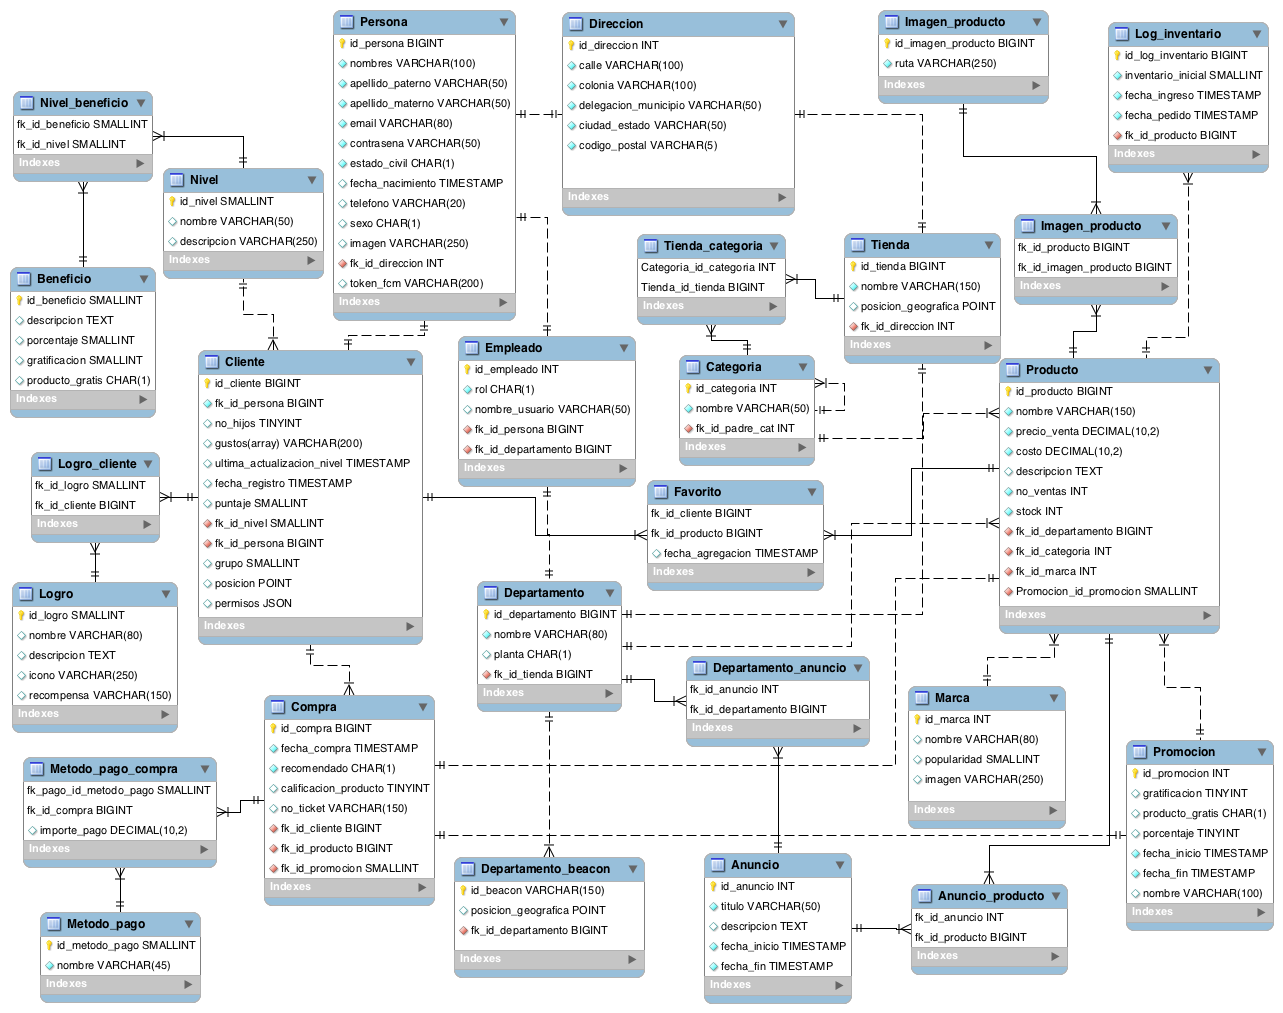
\includegraphics[width=1 \textwidth]{imagenes/modeloDatos/modelorelacional}
		\caption{Modelo relacional de base de datos (Visualización completa).}
		\label{image:modelorelacional}
\end{figure}
\FloatBarrier

La figura \ref{image:modelorelacional-parte1} muestra la parte 1 del diagrama.

\FloatBarrier
\begin{figure}[htbp!]
		\centering
			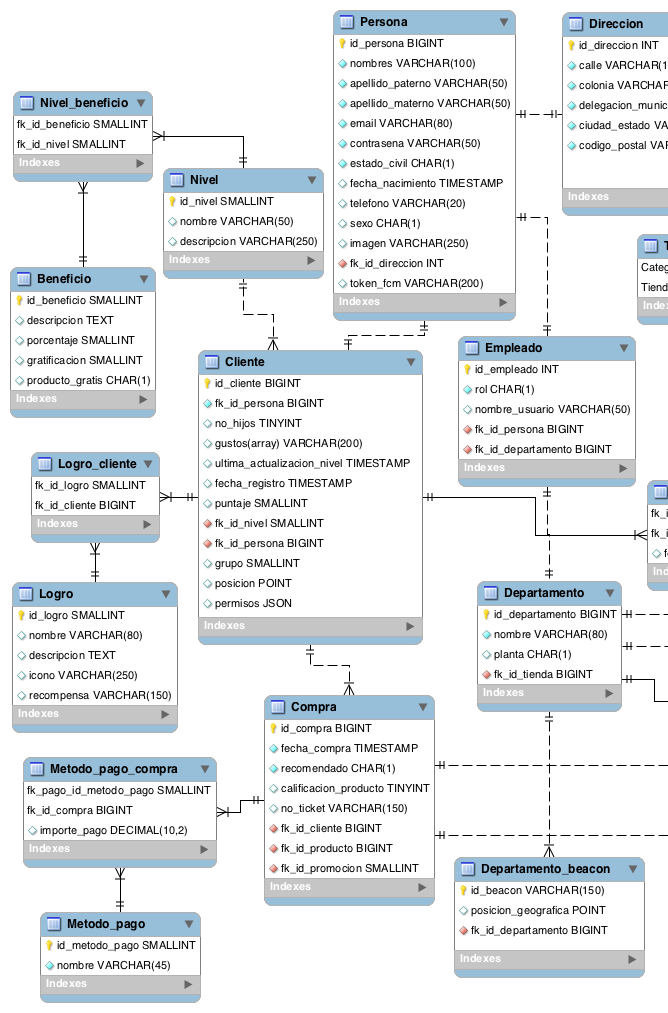
\includegraphics[width=.82 \textwidth]{imagenes/modeloDatos/modelorelacional_1}
		\caption{Modelo relacional de base de datos (Parte 1).}
		\label{image:modelorelacional-parte1}
\end{figure}
\FloatBarrier

La figura \ref{image:modelorelacional-parte2} muestra la parte 2 del diagrama.

\FloatBarrier
\begin{figure}[htbp!]
		\centering
			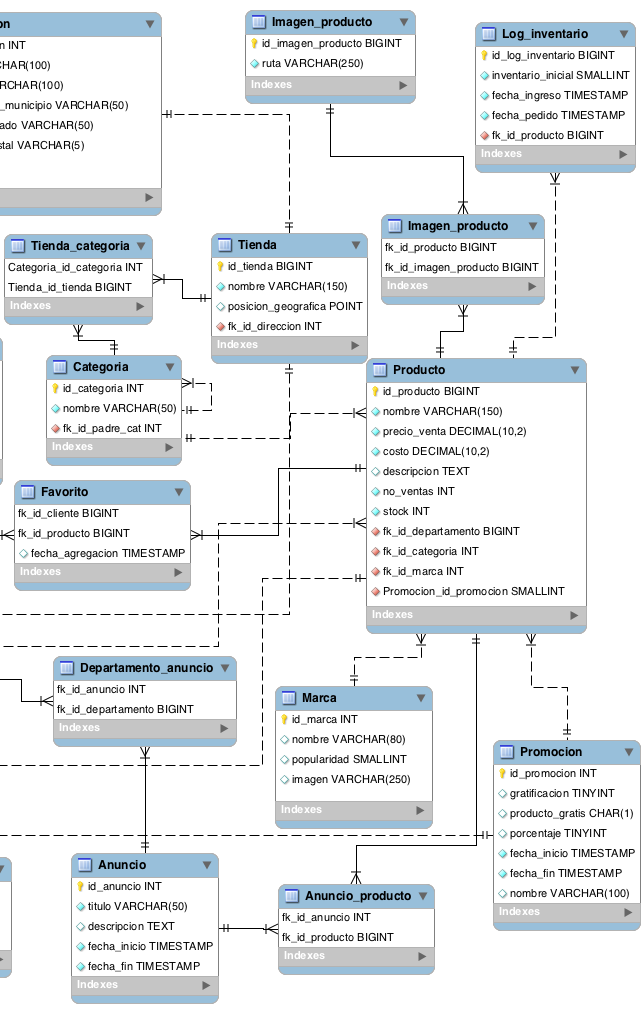
\includegraphics[width=.75 \textwidth]{imagenes/modeloDatos/modelorelacional_2}
		\caption{Modelo relacional de base de datos (Parte 2).}
		\label{image:modelorelacional-parte2}
\end{figure}
\FloatBarrier
 
%---------------------------------------------------------
\section{Prototipo 1: Diseño inicial de la base de datos}
% - - - - - - - - - - - - - - - - - - - - - - - - -
\subsection{Diccionario de datos}
%FALTA COLOCAR EL NÚMERO DE TABLA QUE ES

\cfinput{disenoAplicacion/diccionarioDatos/anuncio}
\cfinput{disenoAplicacion/diccionarioDatos/atributo}
\cfinput{disenoAplicacion/diccionarioDatos/beneficio}
\cfinput{disenoAplicacion/diccionarioDatos/categoria}
\cfinput{disenoAplicacion/diccionarioDatos/cliente}
\cfinput{disenoAplicacion/diccionarioDatos/compra}
\cfinput{disenoAplicacion/diccionarioDatos/departamento_anuncio}
\cfinput{disenoAplicacion/diccionarioDatos/departamento_beacon}
\cfinput{disenoAplicacion/diccionarioDatos/departamento	}
\cfinput{disenoAplicacion/diccionarioDatos/direccion_persona}
\cfinput{disenoAplicacion/diccionarioDatos/empleado}
\cfinput{disenoAplicacion/diccionarioDatos/favorito}
\cfinput{disenoAplicacion/diccionarioDatos/imagen}
\cfinput{disenoAplicacion/diccionarioDatos/log_inventario}
\cfinput{disenoAplicacion/diccionarioDatos/logro_cliente}
\cfinput{disenoAplicacion/diccionarioDatos/logro}
\cfinput{disenoAplicacion/diccionarioDatos/marca}
\cfinput{disenoAplicacion/diccionarioDatos/metodo_pago_compra}
\cfinput{disenoAplicacion/diccionarioDatos/metodo_pago}
\cfinput{disenoAplicacion/diccionarioDatos/nivel_beneficio}
\cfinput{disenoAplicacion/diccionarioDatos/nivel}
\cfinput{disenoAplicacion/diccionarioDatos/persona}
\cfinput{disenoAplicacion/diccionarioDatos/producto_anuncio}
\cfinput{disenoAplicacion/diccionarioDatos/producto_atributo}
\cfinput{disenoAplicacion/diccionarioDatos/producto_imagen}
\cfinput{disenoAplicacion/diccionarioDatos/producto}
\cfinput{disenoAplicacion/diccionarioDatos/promocion}
\cfinput{disenoAplicacion/diccionarioDatos/tienda}
\cfinput{disenoAplicacion/diccionarioDatos/tipo_atributo}

%---
% - - - - - - - - - - - - - - - - - - - - - - - - -
\subsection{Modelo de la base de datos}
La figura \ref{image:prototipo1basededatos1} mostrada en la parte inferior, presenta el  de la base de datos que esta compuesto por cada una de las entidades definidas anteriormente y que permite visualizar adecuadamente la conexión entre cada una de ellas.
Este diagrama se ha dividido en dos secciones a fin de poder obtener una mejor visualización de los datos, las figuras posteriores \ref{image:prototipo1basededatos2} y \ref{image:prototipo1basededatos3} son dichas divisiones de la figura \ref{image:prototipo1basededatos1}.
\label{Modelo-BD}
\FloatBarrier
\begin{figure}[htbp!]
		\centering
			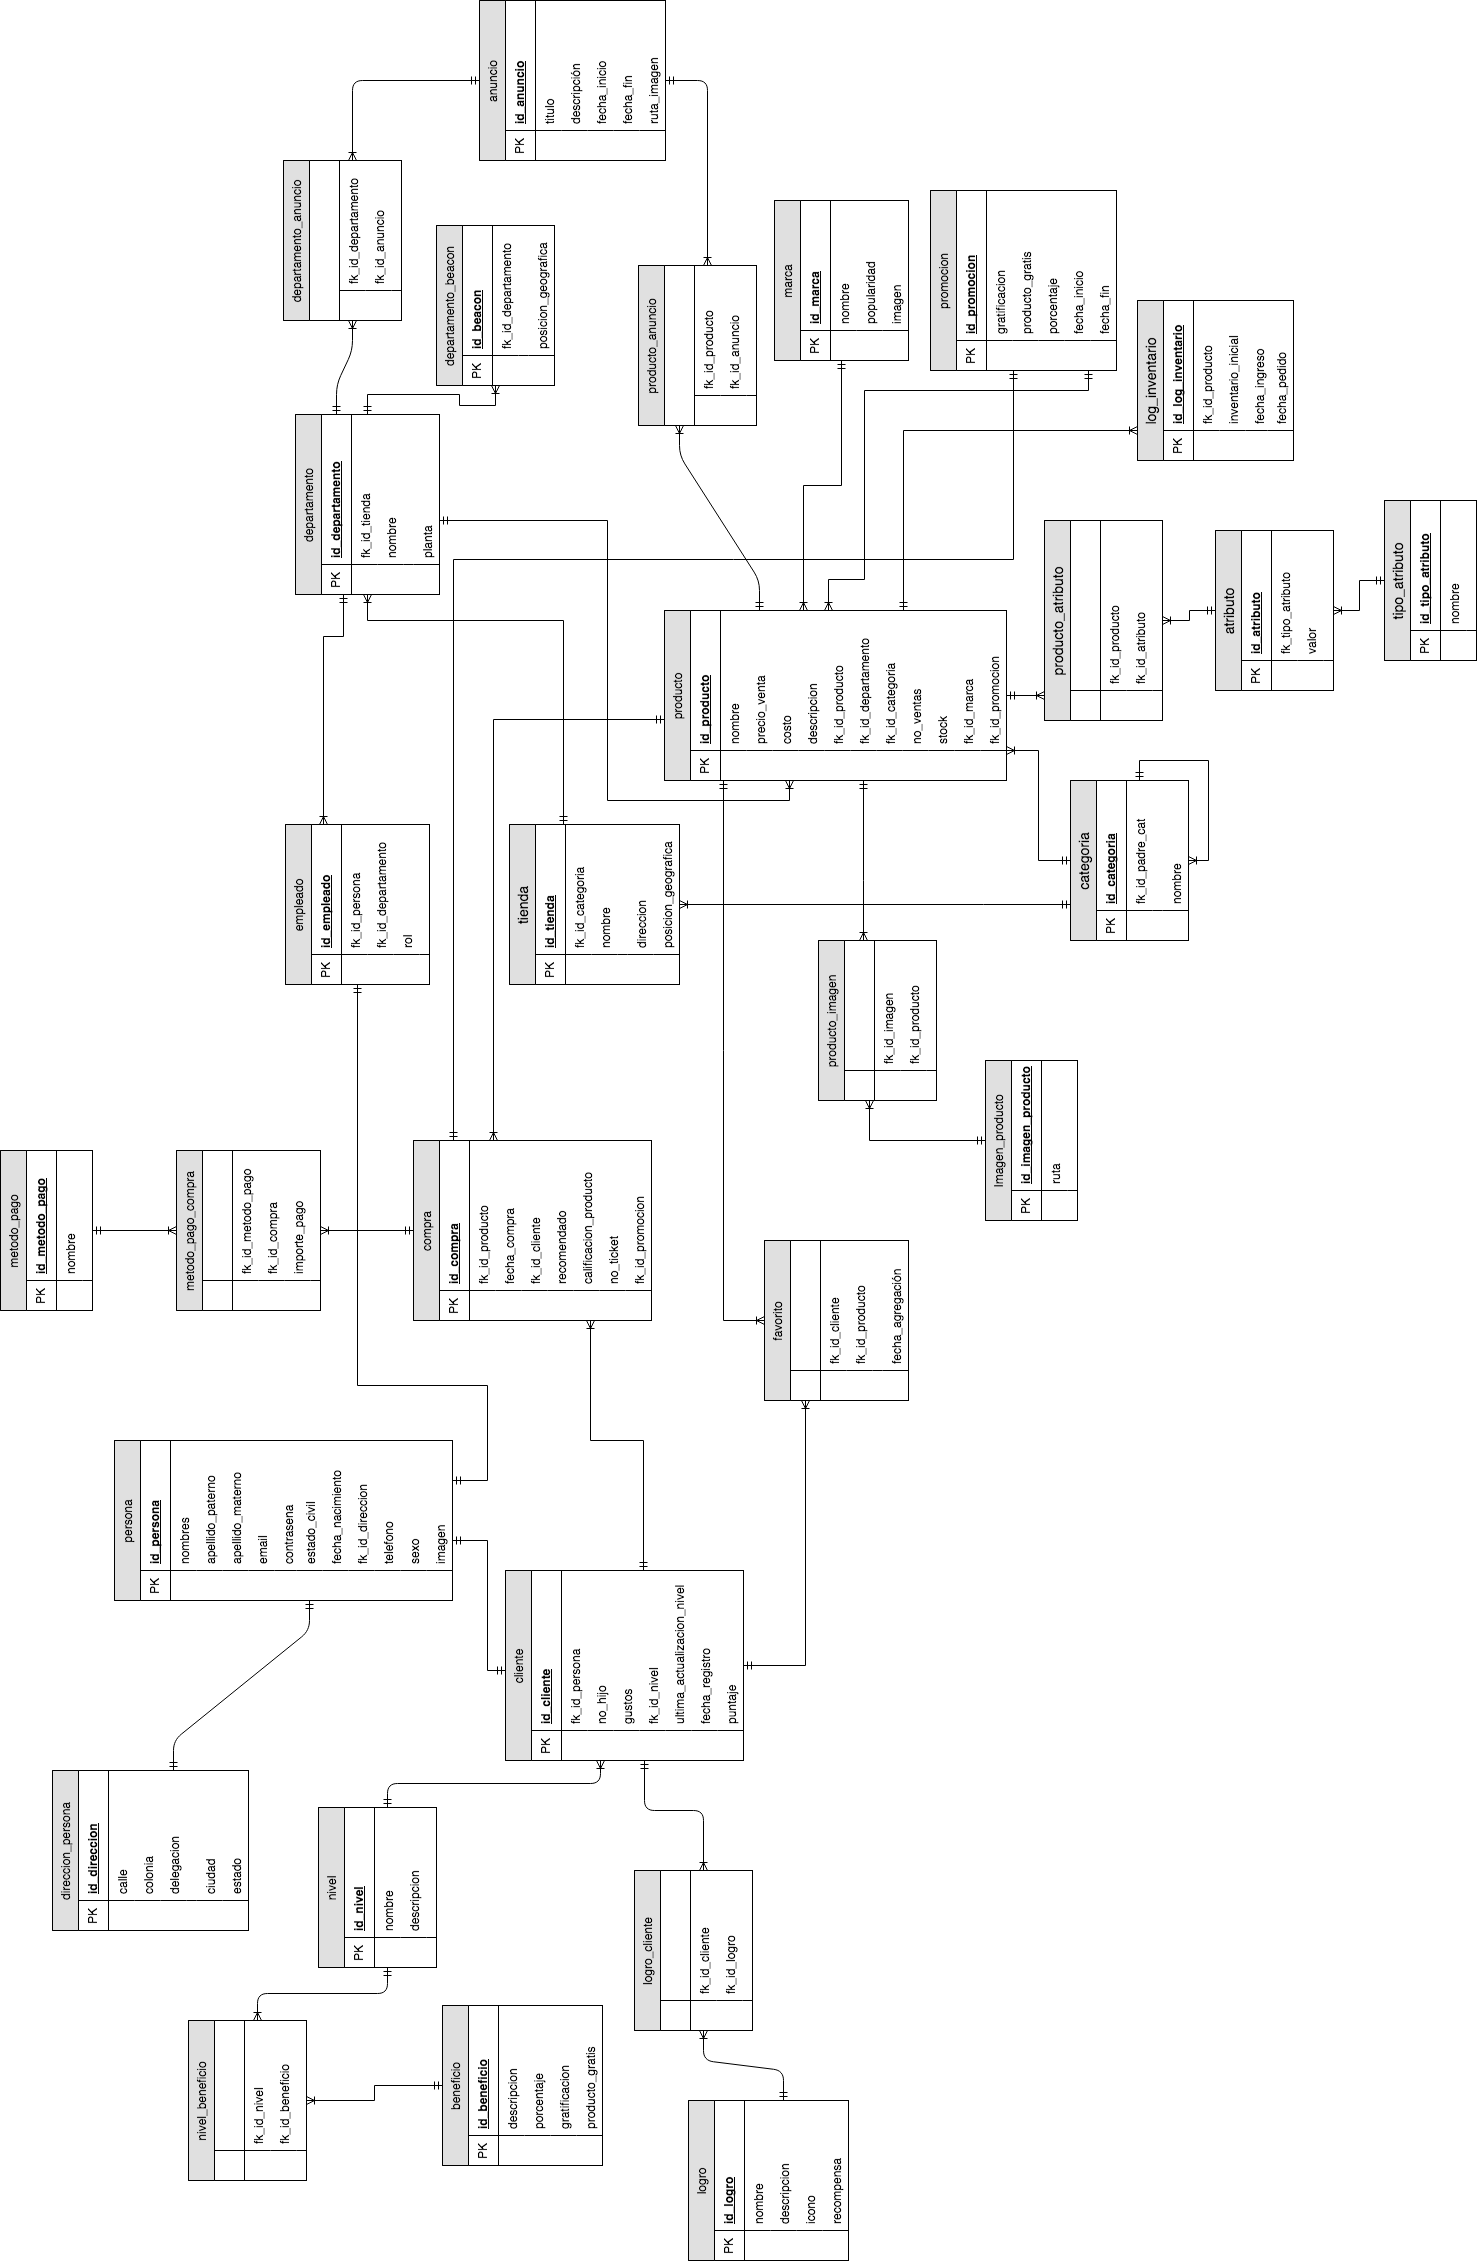
\includegraphics[width=.9 \textwidth]{images/TT_database_1}
		\caption{Prototipo 1: Diagrama del modelo de la base de datos (Visualización completa).}
		\label{image:prototipo1basededatos1}
\end{figure}
\FloatBarrier

\FloatBarrier
\begin{figure}[htbp!]
		\centering
			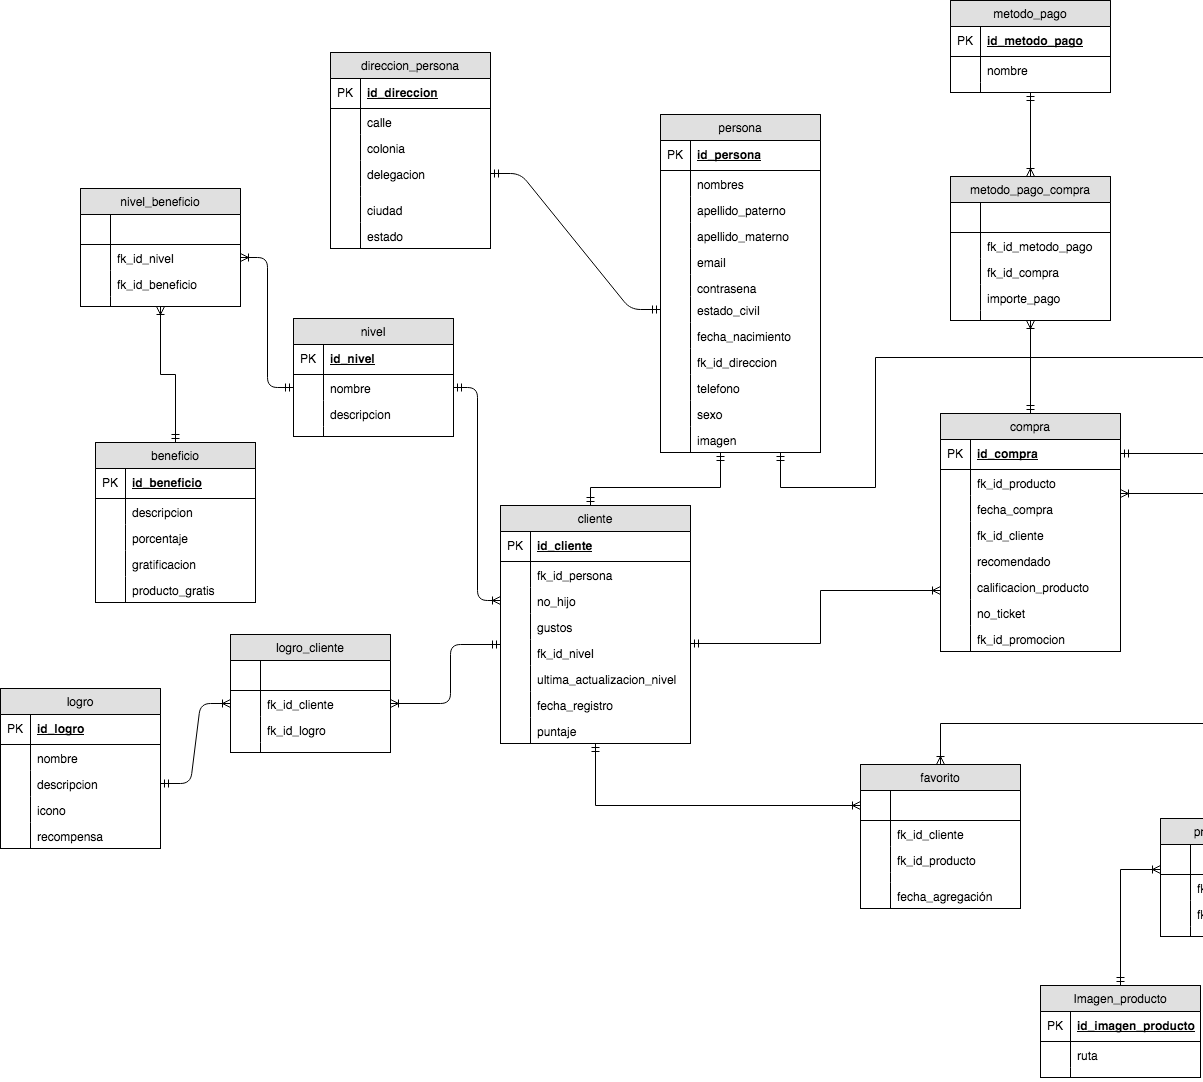
\includegraphics[width=1 \textwidth]{images/TT_database_parte1}
		\caption{Prototipo 1: Diagrama del modelo de la base de datos (Parte 1).}
		\label{image:prototipo1basededatos2}
\end{figure}
\FloatBarrier

\FloatBarrier
\begin{figure}[htbp!]
		\centering
			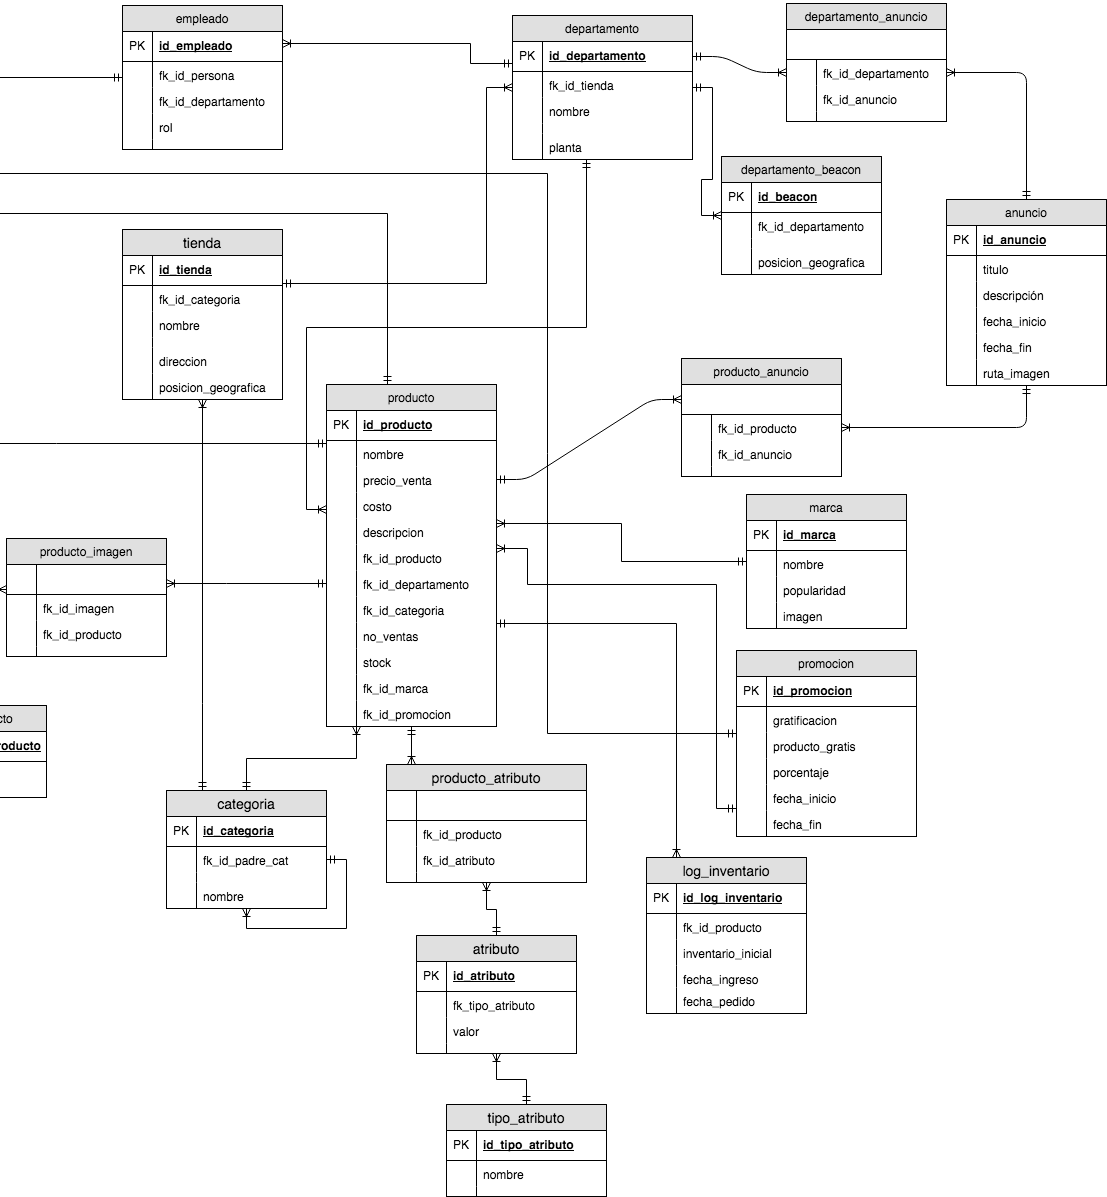
\includegraphics[width=1 \textwidth]{images/TT_database_parte2}
		\caption{Prototipo 1: Diagrama del modelo de la base de datos (Parte 2).}
		\label{image:prototipo1basededatos3}
\end{figure}
\FloatBarrier

\section{Prototipo 1.1: Modificaciones al modelo de la base de datos}

A continuación se muestran enlistados los cambios realizados al modelo de la base de datos anterior, de igual manera se muestra el diccionario de datos para las entidades que fueron modificadas y posteriormente se observa el diagrama con las correcciones correspondientes. 
\\ \par
\subsection{Modificaciones realizadas}
\begin{itemize}
\item Se cambió la entidad \textbf{direccion\_persona} a \textbf{direccion}.
\item Dentro de la entidad \textbf{direccion} se realizaron las siguientes modificaciones:
\begin{itemize}
\item Se borró el campo calle.
\item Se cambió de nombre el campo \textbf{delegacion} a \textbf{delegacion\_municipio}.
\item Se cambió de nombre el campo \textbf{estado} a \textbf{ciudad\_estado}.
\item Se agregó el campo \textbf{codigo\_postal} de tipo \textit{varchar(7)}.
\end{itemize}
\item Se agregó llave foranea \textbf{fk\_id\_direccion} a la entidad \textbf{tienda} con referencia  \textbf{direccion(id\_direccion)}.
\item Se agregó campo \textbf{nombre} a la entidad \textbf{promocion} con tipo de dato \textit{varchar(100)}.
\item Se modificó la cardinalidad de \textbf{tienda-categoria} a muchos a muchos.
\item Se eliminó el campo \textbf{fk\_id\_producto} de la entidad \textbf{producto}.
\item Se agregó el campo \textbf{nombre\_usuario} a la entidad \textbf{empleado}

\end{itemize}

\subsection{Diccionario de datos}

\cfinput{disenoAplicacion/diccionarioDatos/prototipo1_1/empleado}
\cfinput{disenoAplicacion/diccionarioDatos/prototipo1_1/direccion}
\cfinput{disenoAplicacion/diccionarioDatos/prototipo1_1/promocion}
\cfinput{disenoAplicacion/diccionarioDatos/prototipo1_1/tienda}
\cfinput{disenoAplicacion/diccionarioDatos/prototipo1_1/tienda_categoria}

\subsection{Modelo de la base de datos}

En la figura \ref{image:prototipo11basededatos1}, se puede observar las modificaciones realizadas al modelo de la base de datos, marcadas en color verde para diferenciar las entidades agregadas y en letras negritas los campos modificados o agregados. Este diagrama se ha dividido en dos secciones a fin de poder obtener una mejor visualización de los datos, las figuras posteriores \ref{image:prototipo11basededatos2} y \ref{image:prototipo11basededatos3} son dichas divisiones de la figura \ref{image:prototipo11basededatos1}.
\label{Modelo-BD}
\FloatBarrier
\begin{figure}[htbp!]
		\centering
			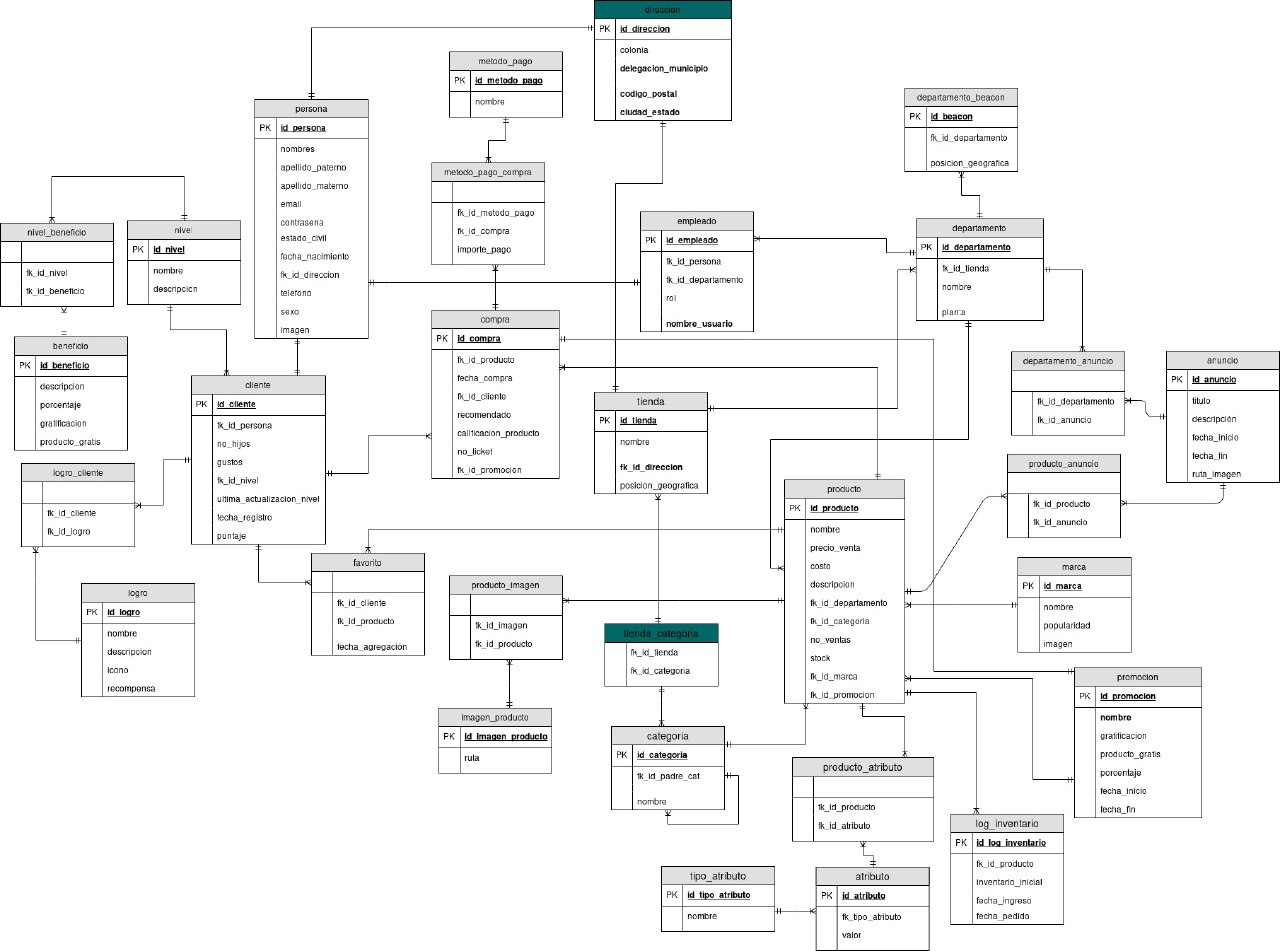
\includegraphics[width=1 \textwidth]{imagenes/modeloDatos/TT_database1_1}
		\caption{Prototipo 1.1: Diagrama del modelo de la base de datos (Visualización completa).}
		\label{image:prototipo11basededatos1}
\end{figure}
\FloatBarrier

\FloatBarrier
\begin{figure}[htbp!]
		\centering
			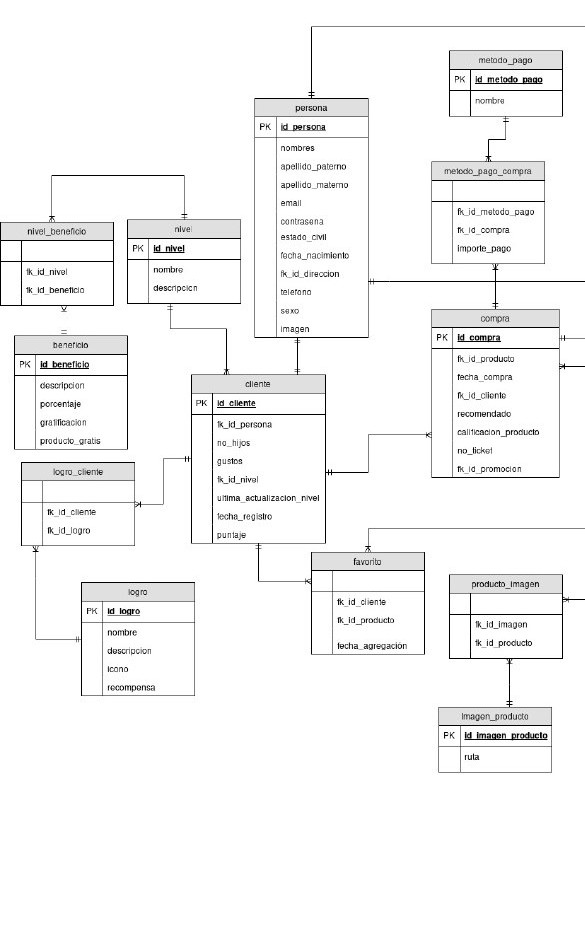
\includegraphics[width=.8 \textwidth]{imagenes/modeloDatos/TT_database1_1_parte1}
		\caption{Prototipo 1.1: Diagrama del modelo de la base de datos (Parte 1).}
		\label{image:prototipo11basededatos2}
\end{figure}
\FloatBarrier

\FloatBarrier
\begin{figure}[htbp!]
		\centering
			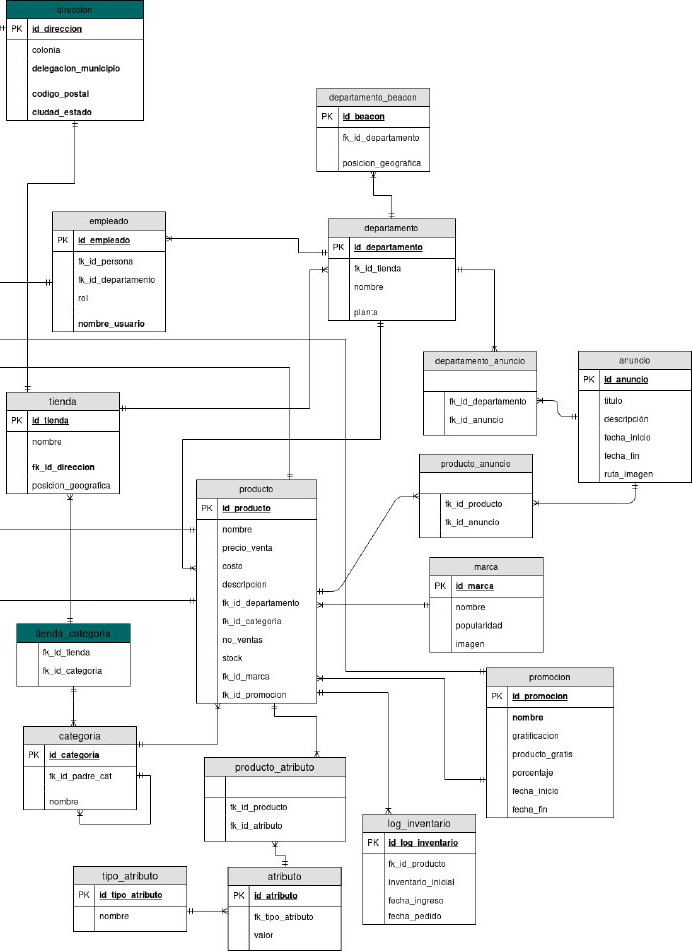
\includegraphics[width=.86 \textwidth]{imagenes/modeloDatos/TT_database1_1_parte2}
		\caption{Prototipo 1.1: Diagrama del modelo de la base de datos (Parte 2).}
		\label{image:prototipo11basededatos3}
\end{figure}
\FloatBarrier


%%%%%% PROTOTIPO 1.2
\section{Prototipo 1.2: Modificaciones al modelo de la base de datos}
En la parte inferior se muestran los cambios realizados al modelo de la base de datos del prototipo 1.1 y de igual manera se muestra el diagrama con dichas modificaciones marcadas sobre él en color rojo las tablas eliminadas y en letras negritas los campos agregados sobre las entidades modificadas.
\\ \par
\subsection{Modificaciones realizadas}
\begin{itemize}
\item Se eliminó la entidad \textbf{producto\_atributo}. 
\item Se eliminó la entidad \textbf{tipo\_atributo}. 
\item Se eliminó la entidad \textbf{atributo}. 
\item Se agregó el campo \textbf{calle} a la entidad \textbf{direccion}
\end{itemize}
\subsection{Diccionario de datos de entidades modificadas}

\cfinput{disenoAplicacion/diccionarioDatos/prototipo1_1/direccion}

\subsection{Modelo de la base de datos}
En la figura \ref{image:prototipo12basededatos1}, se puede observar las modificaciones realizadas al modelo de la base de datos, marcadas nuevamente en color verde para diferenciarlas. Este diagrama se ha dividido en 2 secciones a fin de poder obtener una mejor visualización de los datos, las figuras posteriores \ref{image:prototipo12basededatos2} y \ref{image:prototipo12basededatos3} son dichas divisiones de la figura \ref{image:prototipo12basededatos1}.
\label{Modelo-BD}
\FloatBarrier
\begin{figure}[htbp!]
		\centering
			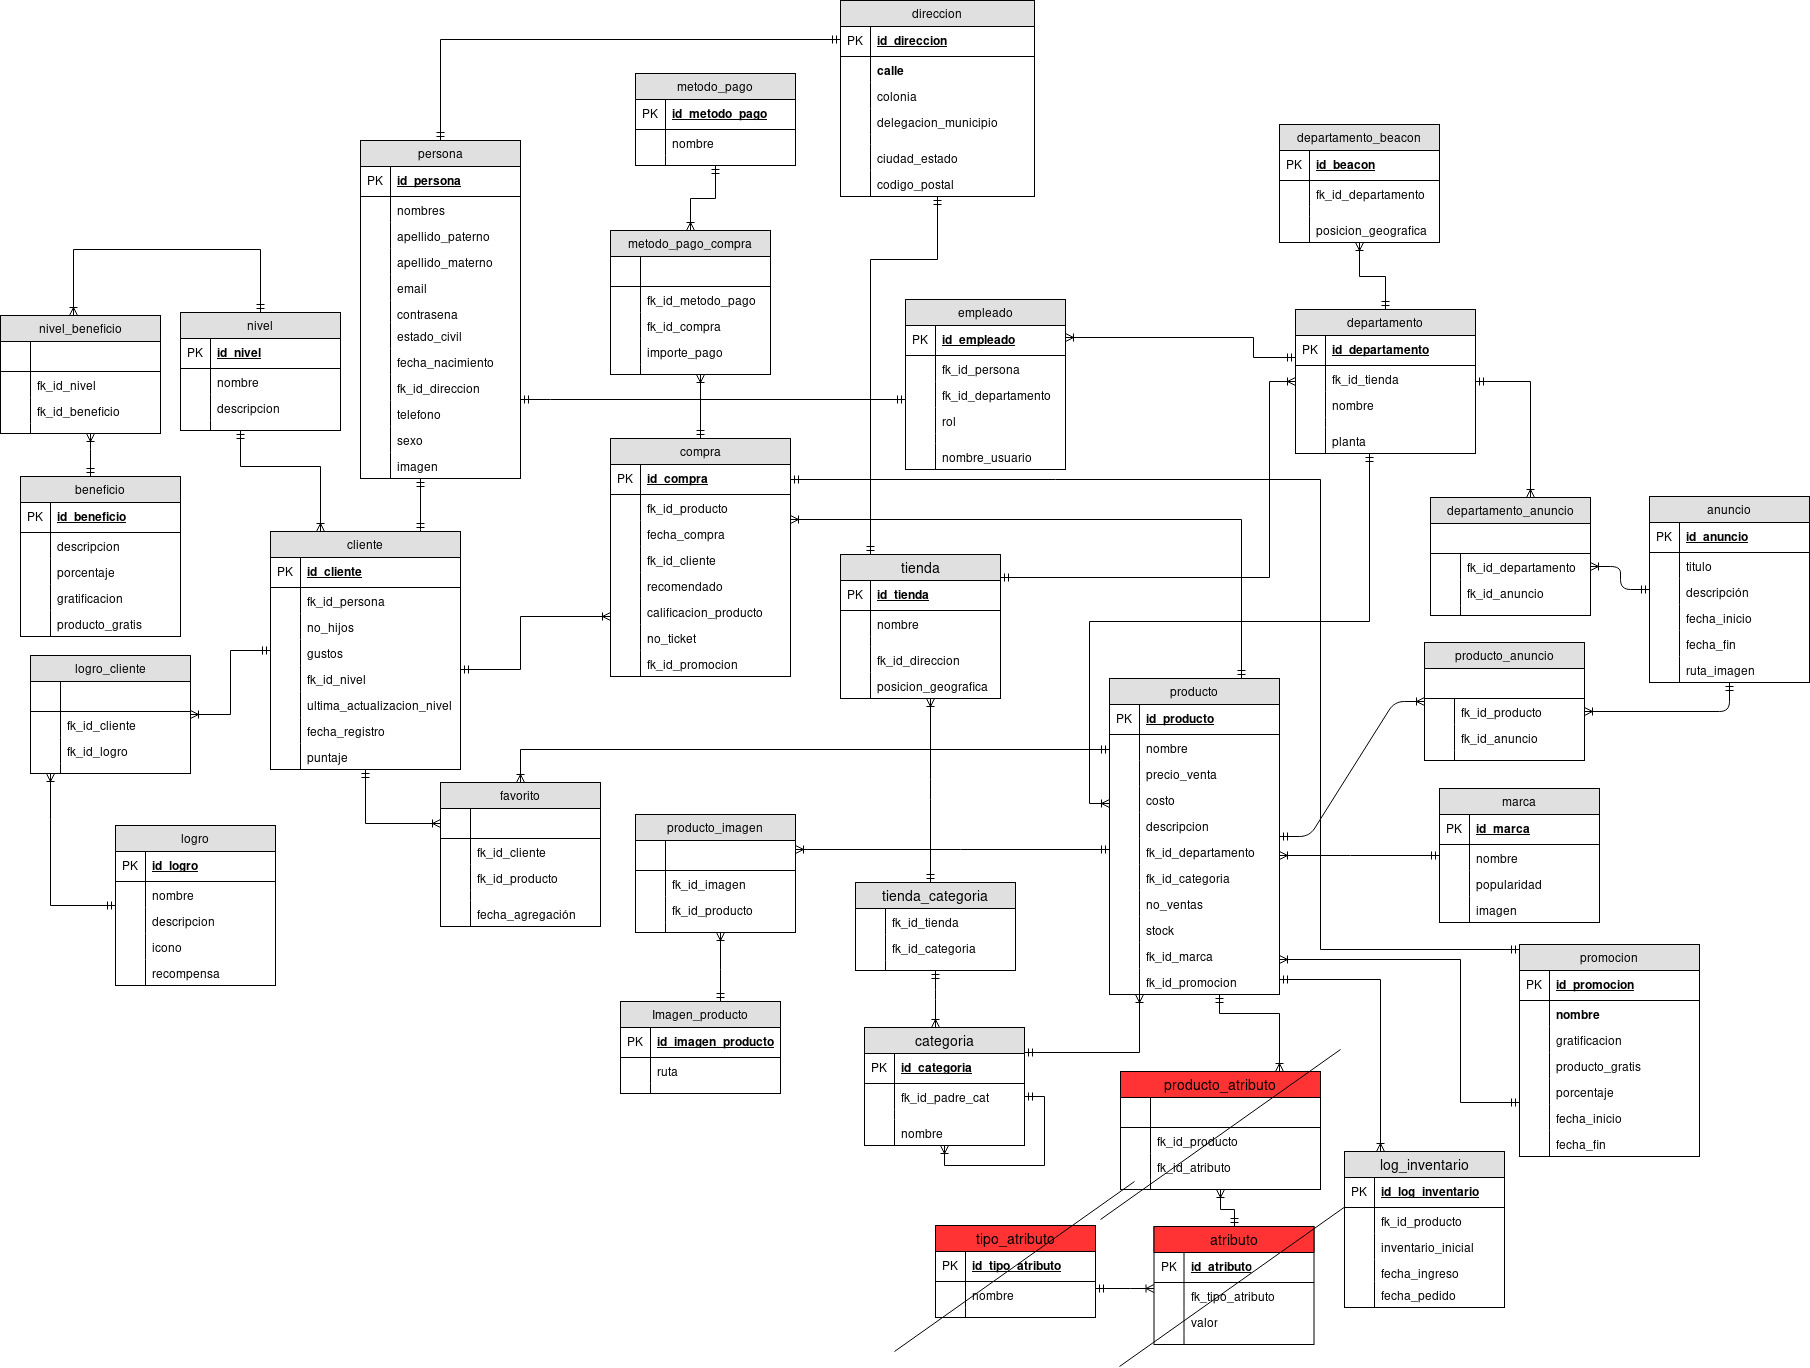
\includegraphics[width=1 \textwidth]{imagenes/modeloDatos/prototipo12/TT_Database_1}
		\caption{Prototipo 1.2: Diagrama del modelo de la base de datos (Visualización completa).}
		\label{image:prototipo12basededatos1}
\end{figure}
\FloatBarrier

\FloatBarrier
\begin{figure}[htbp!]
		\centering
			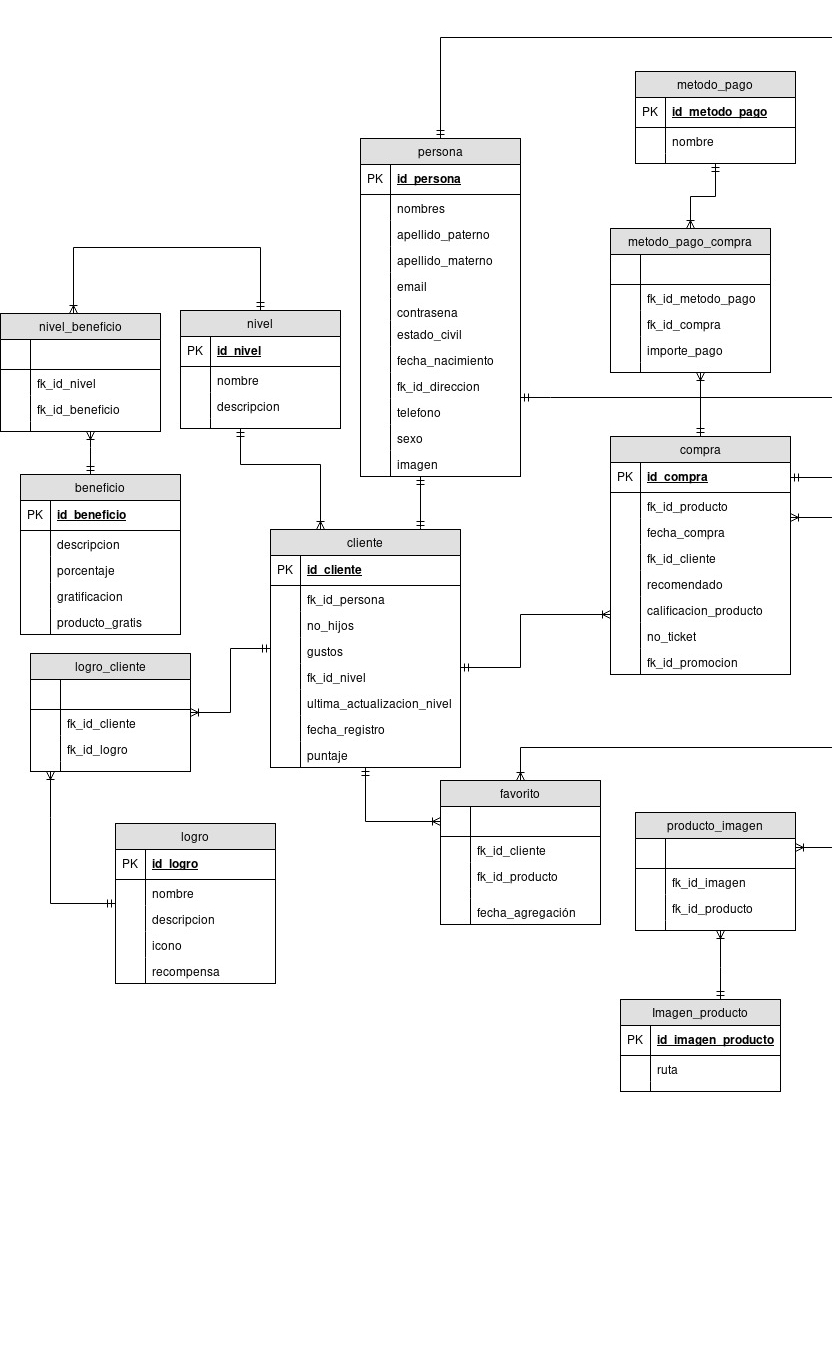
\includegraphics[width=.77 \textwidth]{imagenes/modeloDatos/prototipo12/TT_Database_11_1}
		\caption{Prototipo 1.2: Diagrama del modelo de la base de datos (Parte 1).}
		\label{image:prototipo12basededatos2}
\end{figure}
\FloatBarrier

\FloatBarrier
\begin{figure}[htbp!]
		\centering
			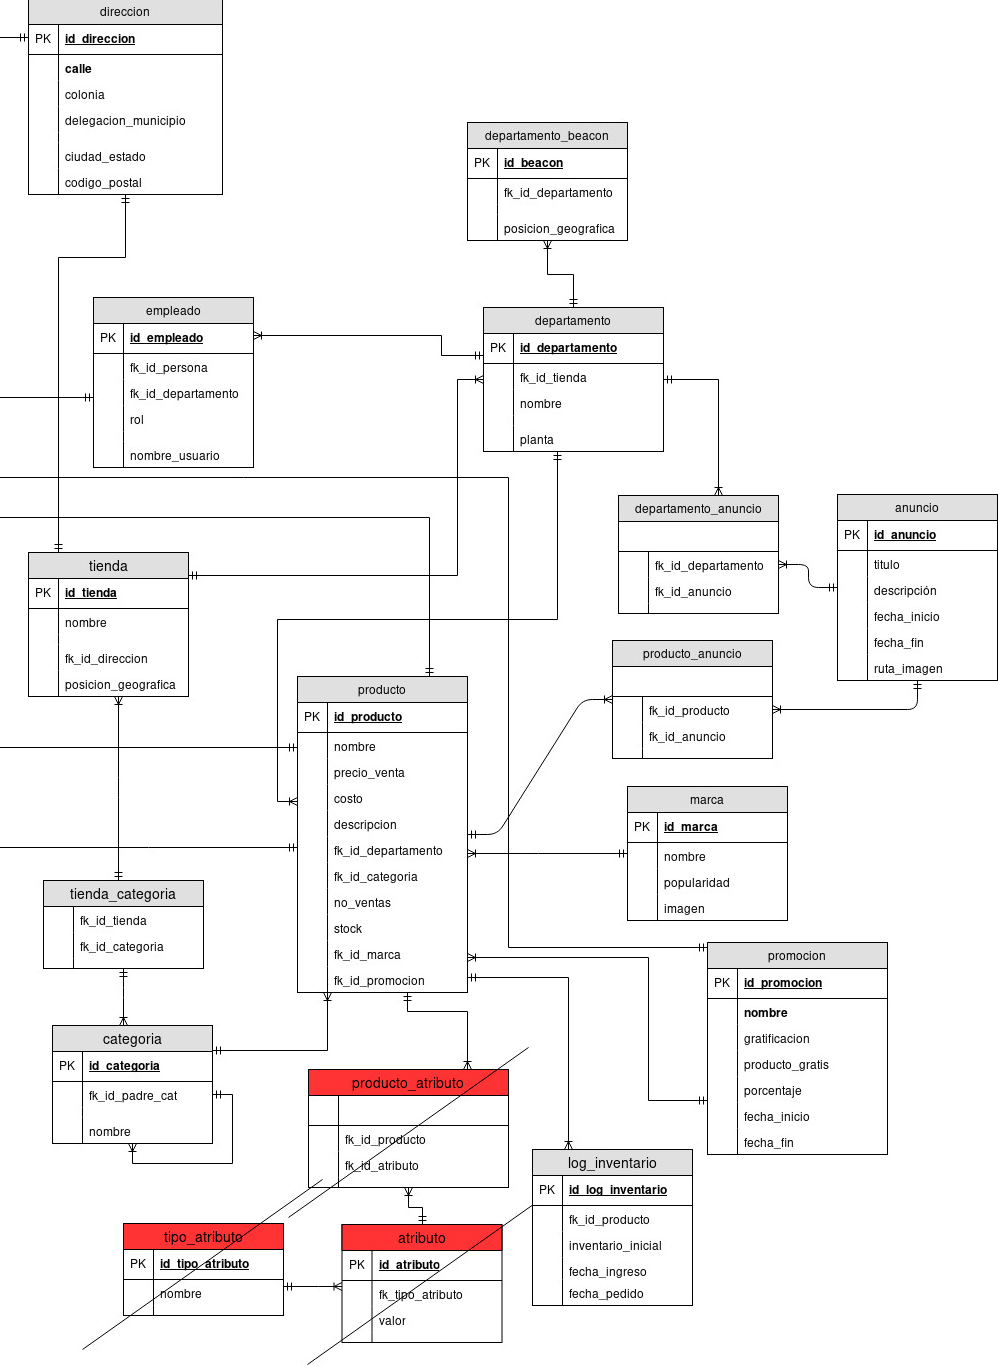
\includegraphics[width=.85 \textwidth]{imagenes/modeloDatos/prototipo12/TT_Database_11_2}
		\caption{Prototipo 1.2: Diagrama del modelo de la base de datos (Parte 2).}
		\label{image:prototipo12basededatos3}
\end{figure}
\FloatBarrier



%%%% PROTOTIPO 1.3
\section{Prototipo 1.3: Modificaciones al modelo de la base de datos}
En la parte inferior se muestran los cambios realizados al modelo de la base de datos del prototipo 1.2 y de igual manera se muestra el diagrama con dichas modificaciones marcadas sobre él en color rojo las tablas eliminadas y verde con letras negritas los campos agregados sobre las entidades modificadas.

\subsection{Modificaciones realizadas}
\begin{itemize}
\item Se agregó el campo \textbf{fecha\_sincronizacion} a la entidad \textbf{departamento\_beacon}
\end{itemize}
\subsection{Diccionario de datos de entidades modificadas}
\cfinput{disenoAplicacion/diccionarioDatos/prototipo1_3/departamento_beacon}


\subsection{Modelo de la base de datos}
En la figura \ref{image:prototipo13basededatos1}, se puede observar las modificaciones realizadas al modelo de la base de datos, marcadas nuevamente en color verde para diferenciarlas. Este diagrama se ha dividido en 2 secciones a fin de poder obtener una mejor visualización de los datos, las figuras posteriores \ref{image:prototipo13basededatos2} y \ref{image:prototipo13basededatos3} son dichas divisiones de la figura \ref{image:prototipo13basededatos1}.
\label{Modelo-BD}
\FloatBarrier
\begin{figure}[htbp!]
		\centering
			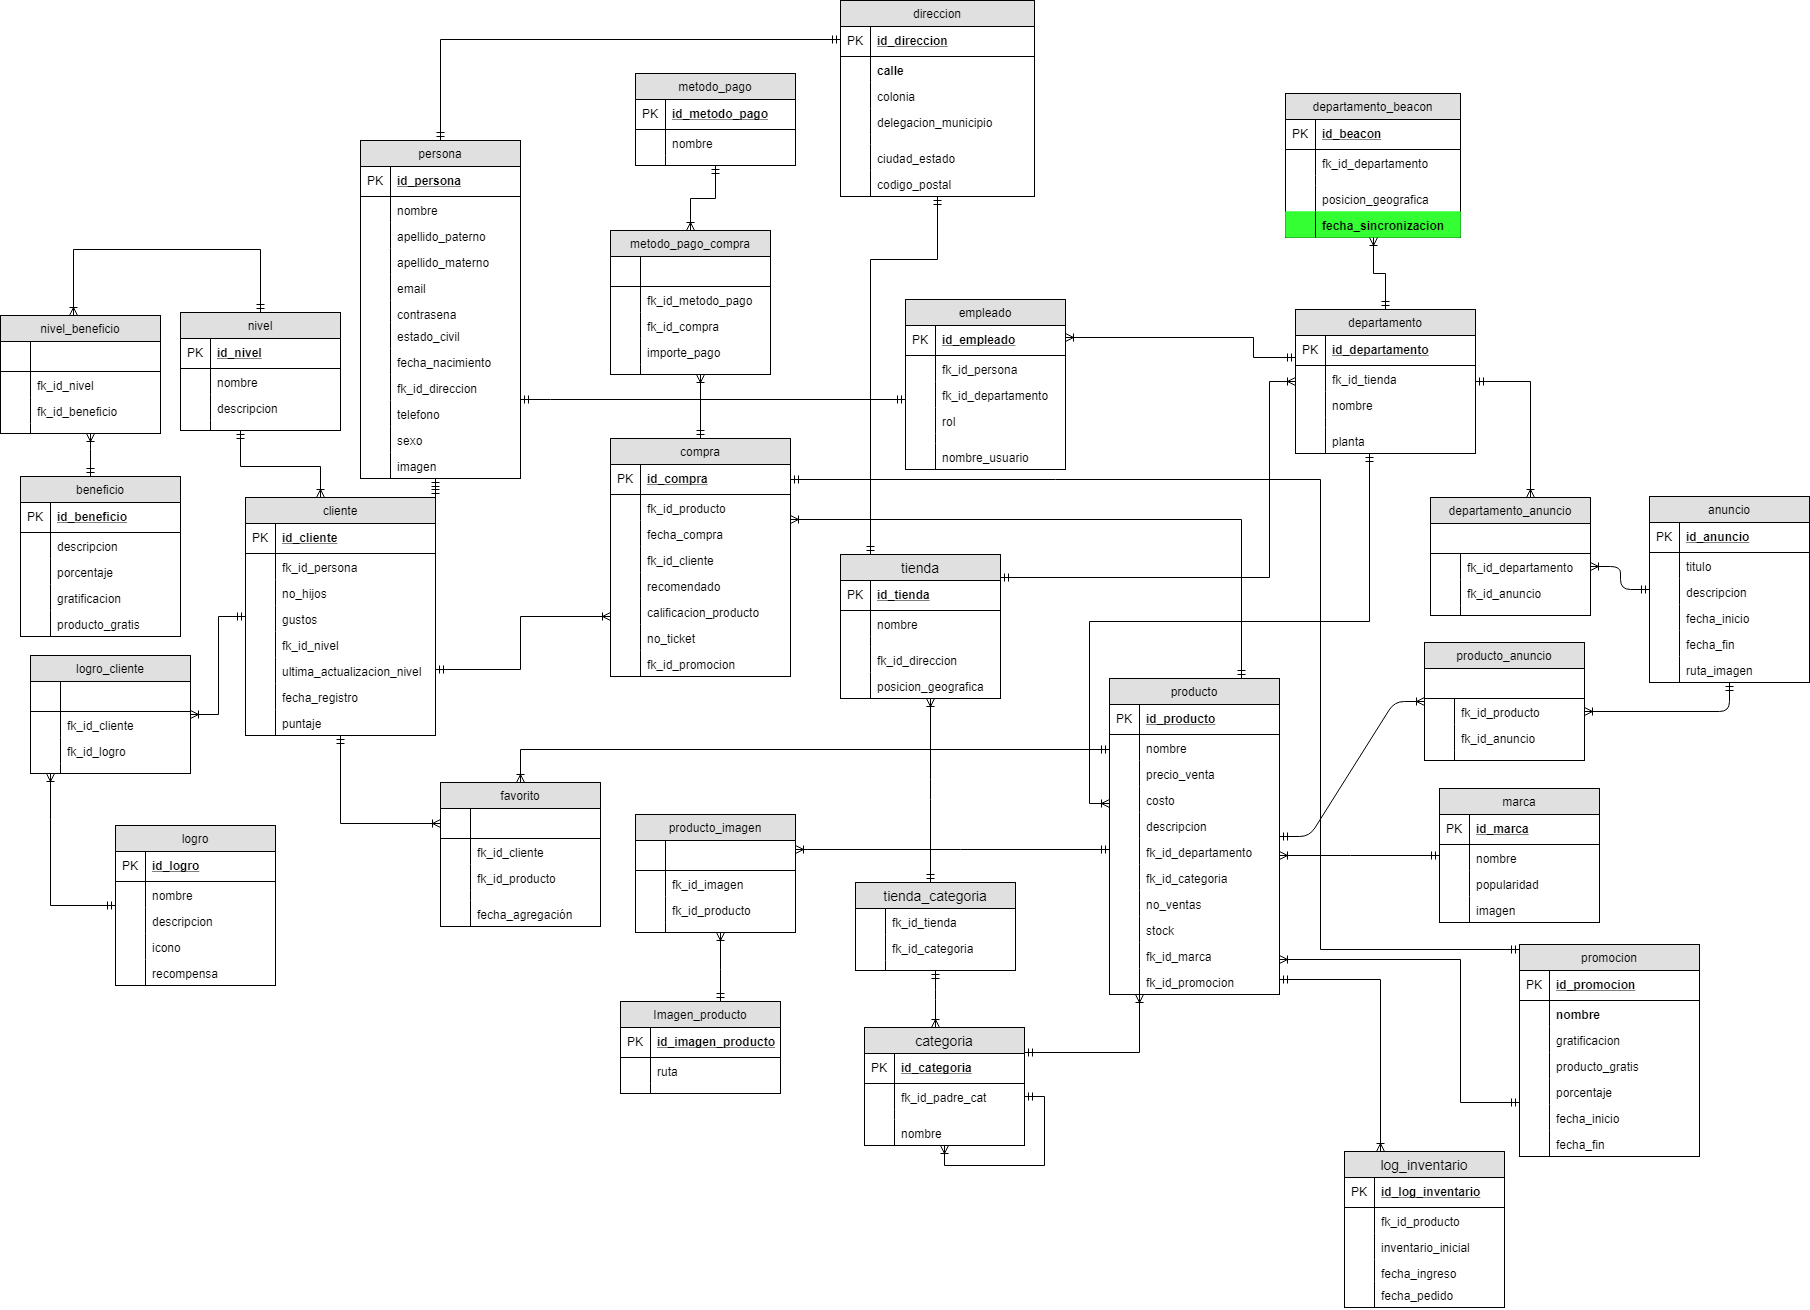
\includegraphics[width=.9 \textwidth]{imagenes/modeloDatos/prototipo13/TT_Database_1}
		\caption{Prototipo 1.3: Diagrama del modelo de la base de datos (Visualización completa).}
		\label{image:prototipo13basededatos1}
\end{figure}
\FloatBarrier

\FloatBarrier
\begin{figure}[htbp!]
		\centering
			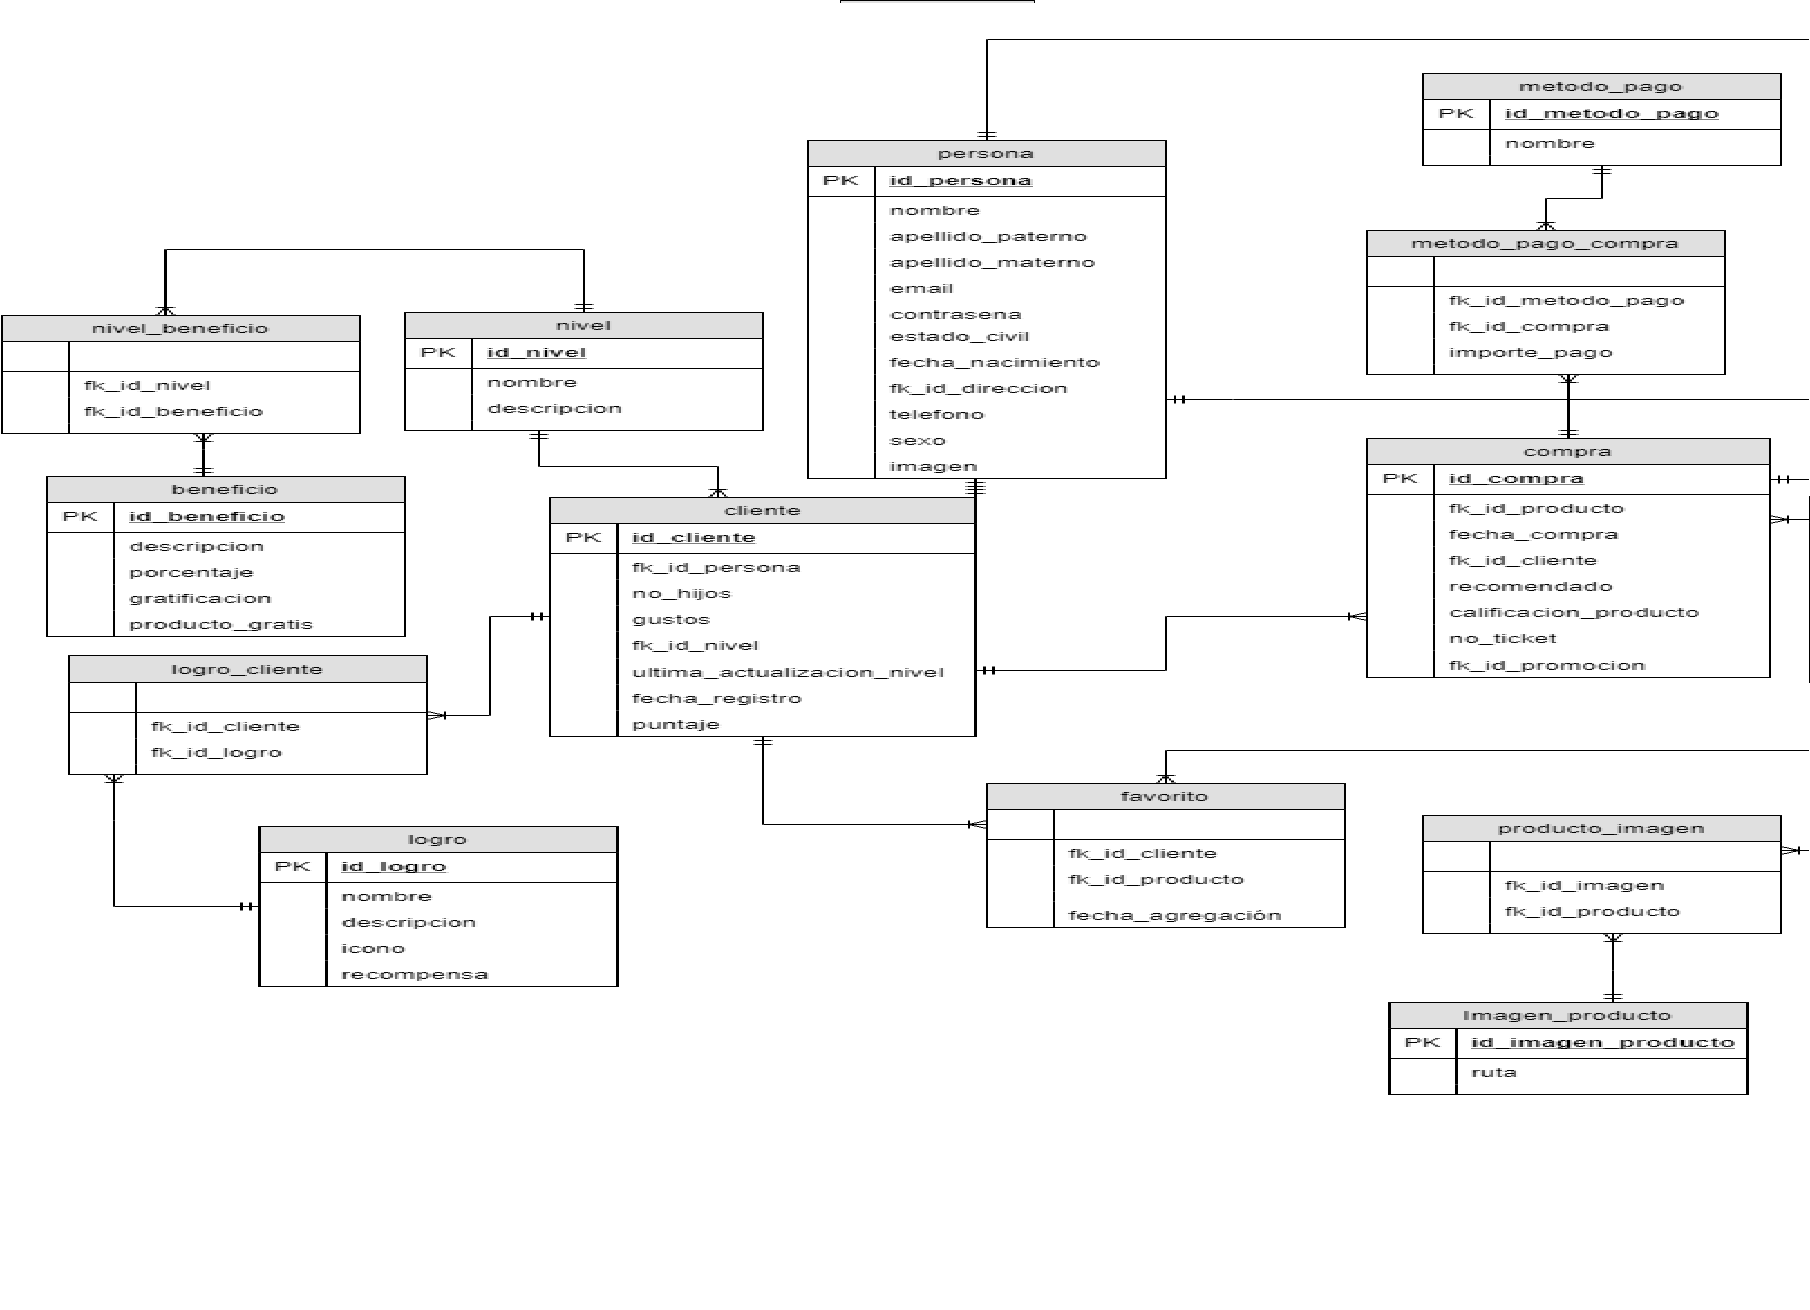
\includegraphics[width=1 \textwidth]{imagenes/modeloDatos/prototipo13/TT_Database_2}
		\caption{Prototipo 1.3: Diagrama del modelo de la base de datos (Parte 1).}
		\label{image:prototipo13basededatos2}
\end{figure}
\FloatBarrier

\FloatBarrier
\begin{figure}[htbp!]
		\centering
			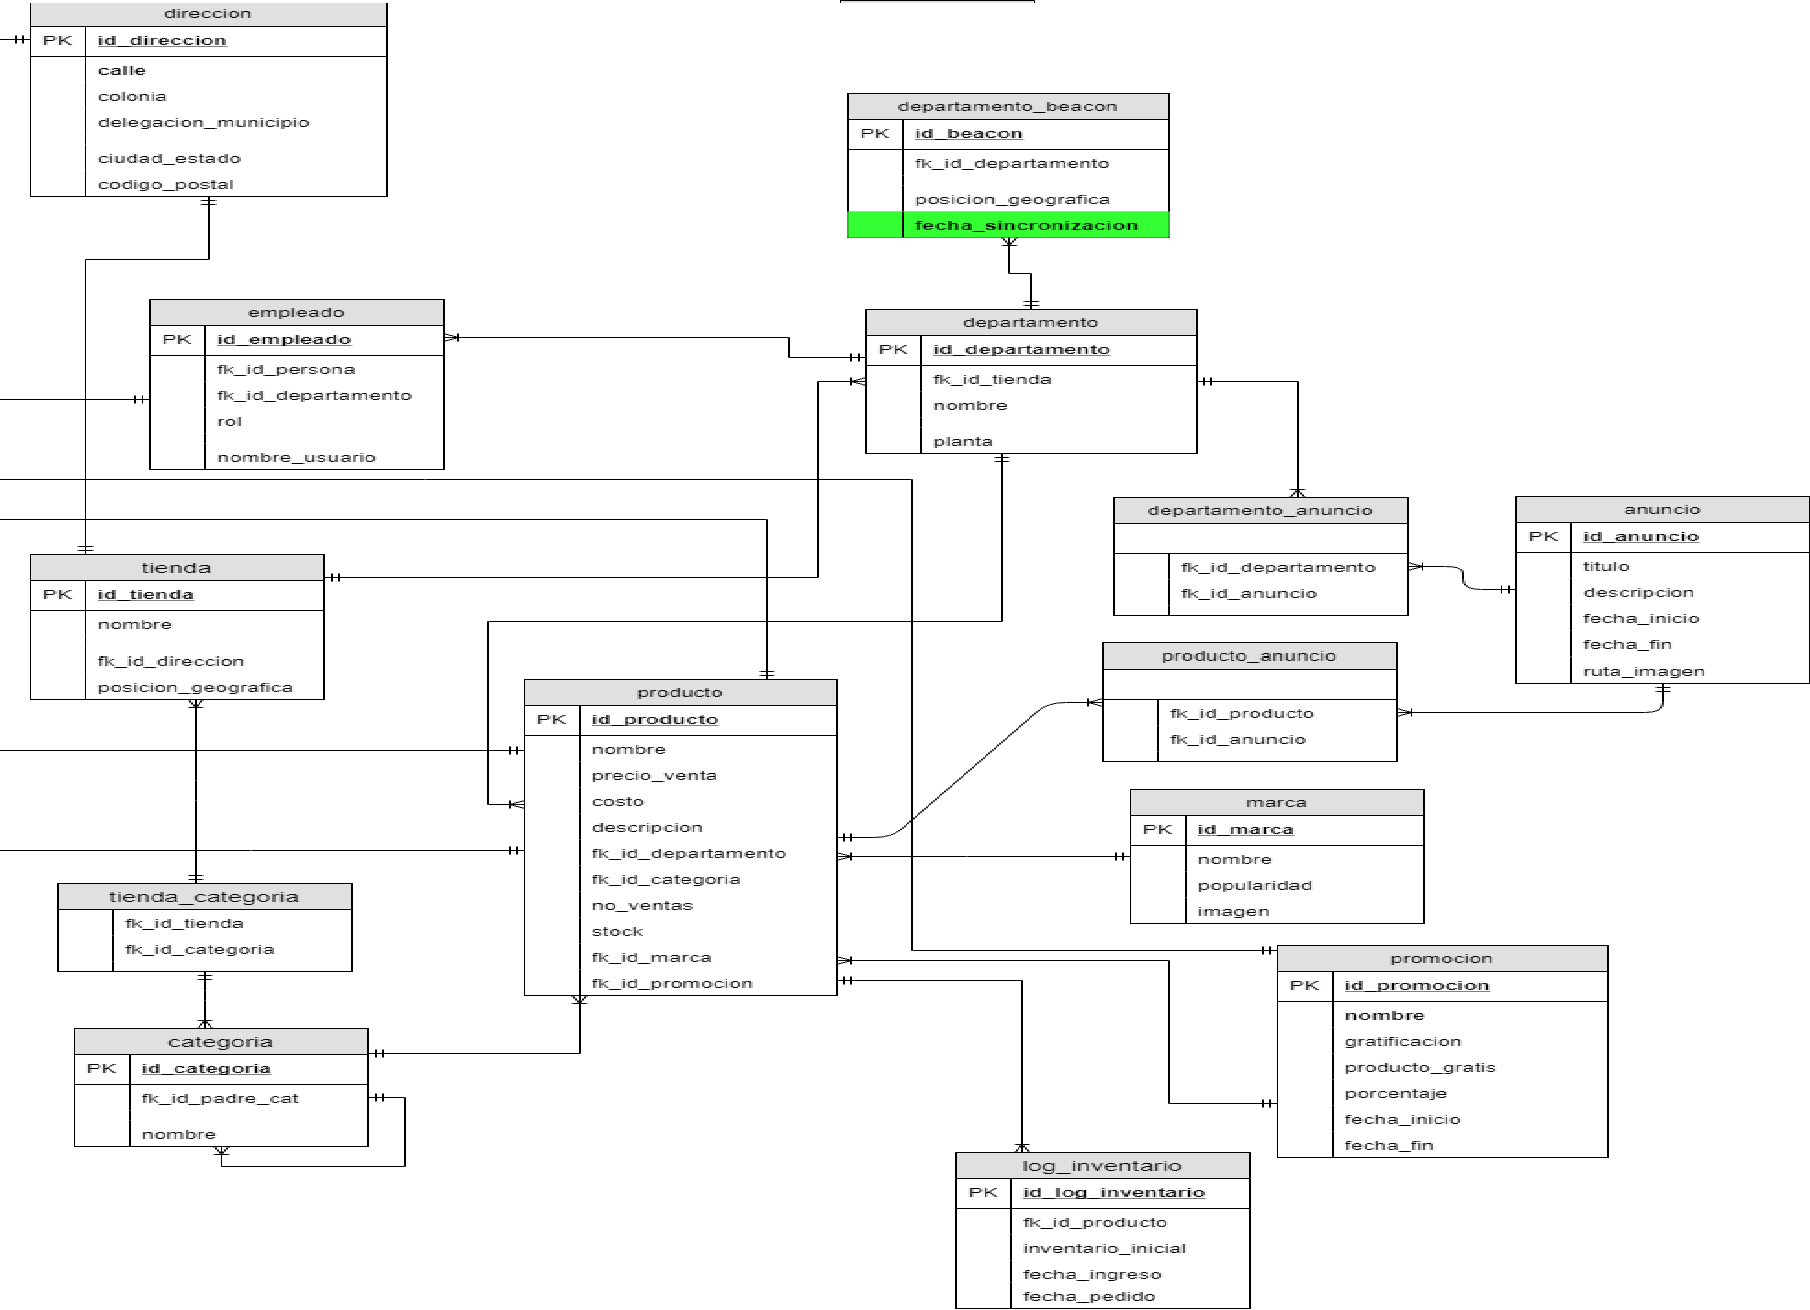
\includegraphics[width=1 \textwidth]{imagenes/modeloDatos/prototipo13/TT_Database_3}
		\caption{Prototipo 1.3: Diagrama del modelo de la base de datos (Parte 2).}
		\label{image:prototipo13basededatos3}
\end{figure}
\FloatBarrier

%%%% PROTOTIPO 1.4
\section{Prototipo 1.4: Modificaciones al modelo de la base de datos}
En la parte inferior se muestran los cambios realizados al modelo de la base de datos del prototipo 1.3 y de igual manera se muestra el diagrama con dichas modificaciones marcadas en fondo verde y letras negritas con los campos agregados sobre las entidades modificadas.

\subsection{Modificaciones realizadas}
\begin{itemize}
\item Se agregó el campo \textbf{token\_fcm} a la entidad \textbf{persona}.
\item Se agregó el campo \textbf{grupo} a la entidad \textbf{cliente}.
\item Se agregó el campo \textbf{posicion} a la entidad \textbf{cliente}.
\item Se agregó el campo \textbf{permisos} a la entidad \textbf{cliente}.
\item Se agregó el campo \textbf{thetas} a la entidad \textbf{cliente}.
\item Se agregó el campo \textbf{x} a la entidad \textbf{producto}.
\item Se agregó el campo \textbf{mu} a la entidad \textbf{producto}.
\end{itemize}

\subsection{Diccionario de datos de entidades modificadas}
\cfinput{disenoAplicacion/diccionarioDatos/prototipo1_4/persona}
\cfinput{disenoAplicacion/diccionarioDatos/prototipo1_4/cliente}
\cfinput{disenoAplicacion/diccionarioDatos/prototipo1_4/producto}


\subsection{Modelo de la base de datos}
En la figura \ref{image:prototipo14basededatos1}, se puede observar las modificaciones realizadas al modelo de la base de datos, marcadas nuevamente en color verde para diferenciarlas. Para una mejor visualización del modelo, se dividió en las figuras \ref{image:prototipo14basededatos2} y \ref{image:prototipo14basededatos3} mostradas a continuación.

\label{Modelo-BD}
\FloatBarrier
\begin{figure}[htbp!]
		\centering
			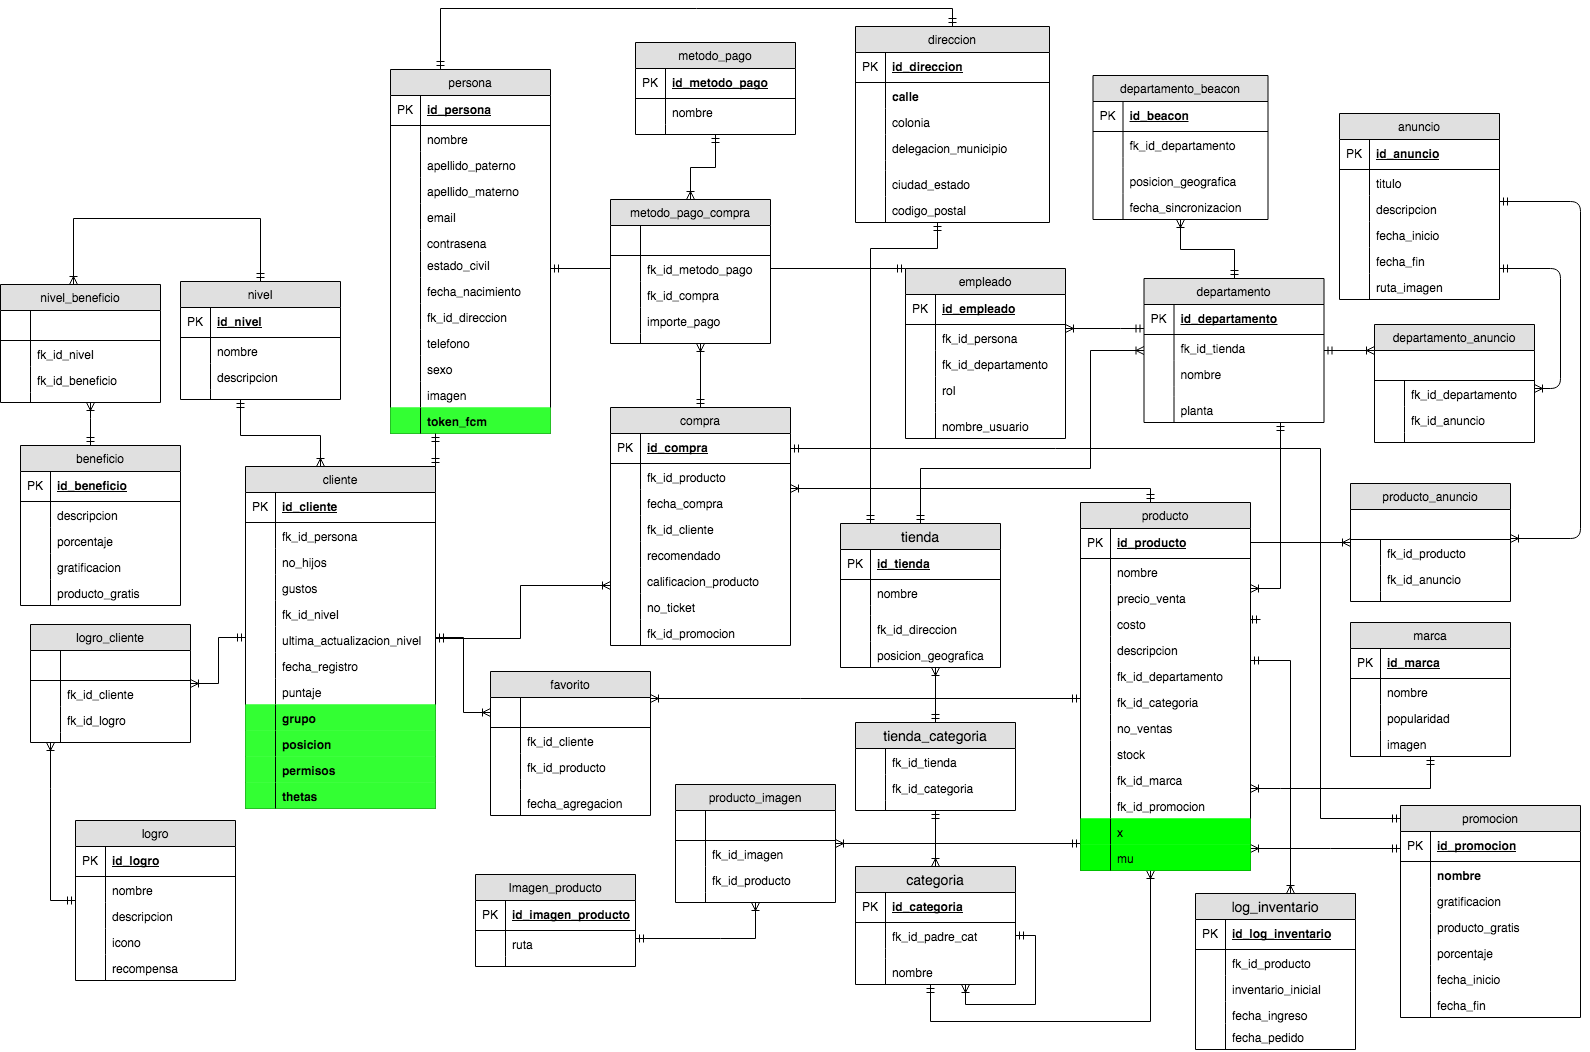
\includegraphics[width=.9 \textwidth]{imagenes/modeloDatos/prototipo14/TT_Database_1}
		\caption{Prototipo 1.4: Diagrama del modelo de la base de datos (Visualización completa).}
		\label{image:prototipo14basededatos1}
\end{figure}
\FloatBarrier

\FloatBarrier
\begin{figure}[htbp!]
		\centering
			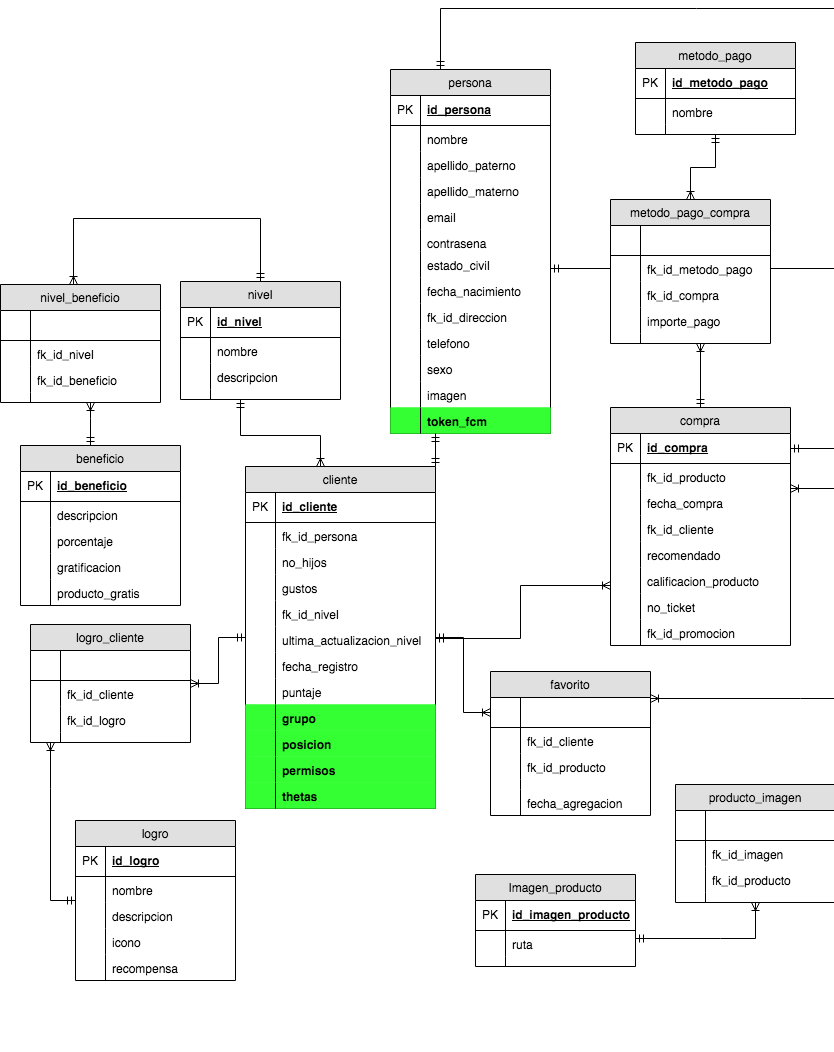
\includegraphics[width=.9 \textwidth]{imagenes/modeloDatos/prototipo14/TT_Database_2}
		\caption{Prototipo 1.4: Diagrama del modelo de la base de datos (Parte 1).}
		\label{image:prototipo14basededatos2}
\end{figure}
\FloatBarrier

\FloatBarrier
\begin{figure}[htbp!]
		\centering
			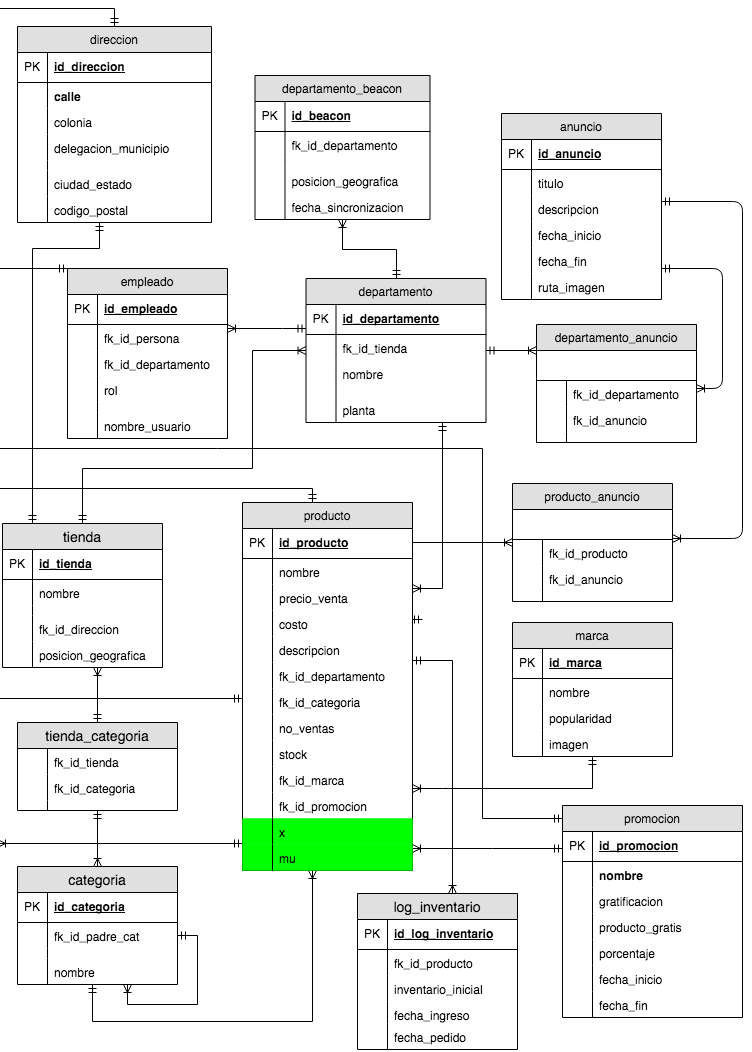
\includegraphics[width=.9 \textwidth]{imagenes/modeloDatos/prototipo14/TT_Database_3}
		\caption{Prototipo 1.4: Diagrama del modelo de la base de datos (Parte 2).}
		\label{image:prototipo14basededatos3}
\end{figure}
\FloatBarrier

%---------------------------------------------------------
%\section{Prototipo 2: Sistema generador de registros artificiales}







